\section{Small-signal modulation response}

\subsection*{Q8: Transfer function from $\VAC$ to $\Delta\phi$}

\paragraph{Linearised force.} With $\Vd(t)=\VDC + \VAC\sin(2\pi f_{m}t)$ and
$\VAC\ll \VDC$, the comb-drive force expands to first order as
\begin{align}
  \Fe &= \tfrac{1}{2}\,(\VDC+\VAC)^{2}\,\frac{dC}{d\xm}
       = \underbrace{\tfrac{1}{2}\VDC^{2}\frac{dC}{d\xm}}_{F_{\mathrm{DC}}}
         \;+\;
         \underbrace{\VDC\,\VAC\,\frac{dC}{d\xm}}_{f_{\mathrm{AC}}(t)}
         \;+\;\mathcal{O}(\VAC^{2}).
\end{align}
The AC component drives the small-signal motion with electromechanical
coupling
\begin{equation}
  \eta \;=\; \VDC\,\frac{dC}{d\xm} \;=\; \VDC\,\frac{N\,\varepsilon_{0}\,t}{h}.
  \label{eq:eta}
\end{equation}
The frequency response of the mass displacement is then
\begin{equation}
  \frac{X(s)}{V_{\!AC}(s)} \;=\; \frac{\eta}{m s^{2} + b s + k},
  \label{eq:Hxv}
\end{equation}
a standard second-order low-pass with poles at the resonance frequency.

\paragraph{Phase-shift sensitivity.} Linearising Eq.~\ref{eq:phase} around
the DC operating gap $g_{\mathrm{op}}=g_{0}+\xm(\VDC)$ via a first-order
Taylor expansion,
\begin{equation}
  \Delta\phi(g_{\mathrm{op}}+\delta g) \;\approx\;
  \Delta\phi(g_{\mathrm{op}})
    + \underbrace{\Bigl.\frac{d\Delta\phi}{dg}\Bigr|_{g_{\mathrm{op}}}}_{\equiv\,S_{\phi}}\,\delta g.
\end{equation}
Using $g=g_{0}+\xm$ so that $\delta g = \delta\xm$, and Eq.~\ref{eq:phase},
\begin{equation}
  \boxed{\;
  S_{\phi} \;=\; \frac{2\pi L}{\lambda}\,
                 (\eta_{\mathrm{eff},0}-\eta_{\mathrm{eff},\infty})\,
                 b\,e^{-b\,g_{\mathrm{op}}}.\;}
\end{equation}

\paragraph{Combined transfer function.} Multiplying Eq.~\ref{eq:Hxv} by
$S_{\phi}$ gives
\begin{equation}
  \boxed{\;
  H(s) \;=\; \frac{\Delta\phi(s)}{V_{\!AC}(s)}
        \;=\; \frac{S_{\phi}\,\eta}{m s^{2} + b s + k}.
  \;}
  \label{eq:Hphi}
\end{equation}

\paragraph{Performance metrics ($\VDC=\SI{10}{\volt}$).}
\begin{align}
  |H|_{f\to 0}     &= \frac{S_{\phi}\,\eta}{k}
                     \;\approx\; \SI{0.40}{\milli\radian\per\volt}, \\[2pt]
  |H|_{f=f_{0}}    &= \frac{S_{\phi}\,\eta\,Q}{k}
                     \;\approx\; \textcolor{blue}{\SI{33}{\milli\radian\per\volt}}
                     \;=\; Q\cdot|H|_{f\to 0}, \\[2pt]
  \text{roll-off} &= -\SI{40}{\decibel\per\text{decade}}\quad
                     \text{(two-pole low-pass above } f_{0}\text{)}.
\end{align}
Fig.~\ref{fig:bode} shows the Bode plot. The magnitude is flat below $f_{0}$,
peaks by $20\log_{10}Q\approx \textcolor{blue}{\SI{38}{\decibel}}$ at the lightly damped
resonance, then rolls off at $-40$\,dB/dec.

\begin{figure}[H]
\centering
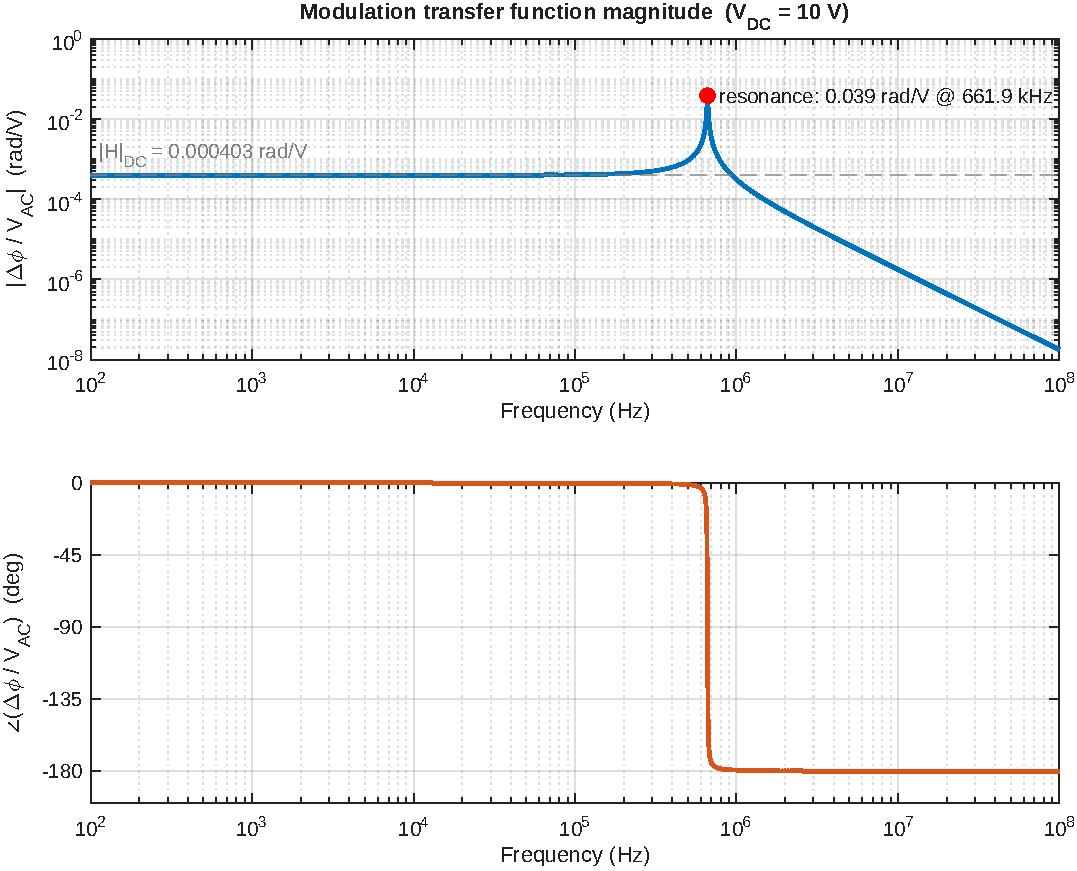
\includegraphics[width=0.85\textwidth]{figures/q8_bode.pdf}
\caption{Bode diagram of the small-signal transfer function
$\Delta\phi(s)/V_{\!AC}(s)$ at $\VDC=\SI{10}{\volt}$. The peak at
$f_{0}\approx\textcolor{blue}{\SI{537}{\kilo\hertz}}$ exceeds the low-frequency value by a
factor of $Q\approx \textcolor{blue}{81}$.}
\label{fig:bode}
\end{figure}

\paragraph{Low-frequency sensitivity vs DC bias.}
From Eqs.~\ref{eq:eta} and \ref{eq:Hphi},
$|H|_{f\to 0} = S_{\phi}\,\VDC\,(N\varepsilon_{0}t/h)/k \propto \VDC$ to first
order. Sensitivity scales linearly with $\VDC$ because $\eta$ does.
Fig.~\ref{fig:sensVDC} shows the response over $\VDC\in[0,\,5]\,\mathrm{kV}$,
with the linear small-signal prediction and the result that includes the
operating-point shift in $S_{\phi}$. Two practical limits are also marked:
finger-tip pull-in at $V_{\mathrm{PI}}\!\approx\!\SI{347}{\volt}$ and
mass-waveguide contact at $\!\approx\!\SI{477}{\volt}$. Above
$\sim\!\SI{350}{\volt}$ the device snaps down, so most of the plotted range
is unreachable in practice, it is shown only to illustrate the trend.

\begin{figure}[H]
\centering
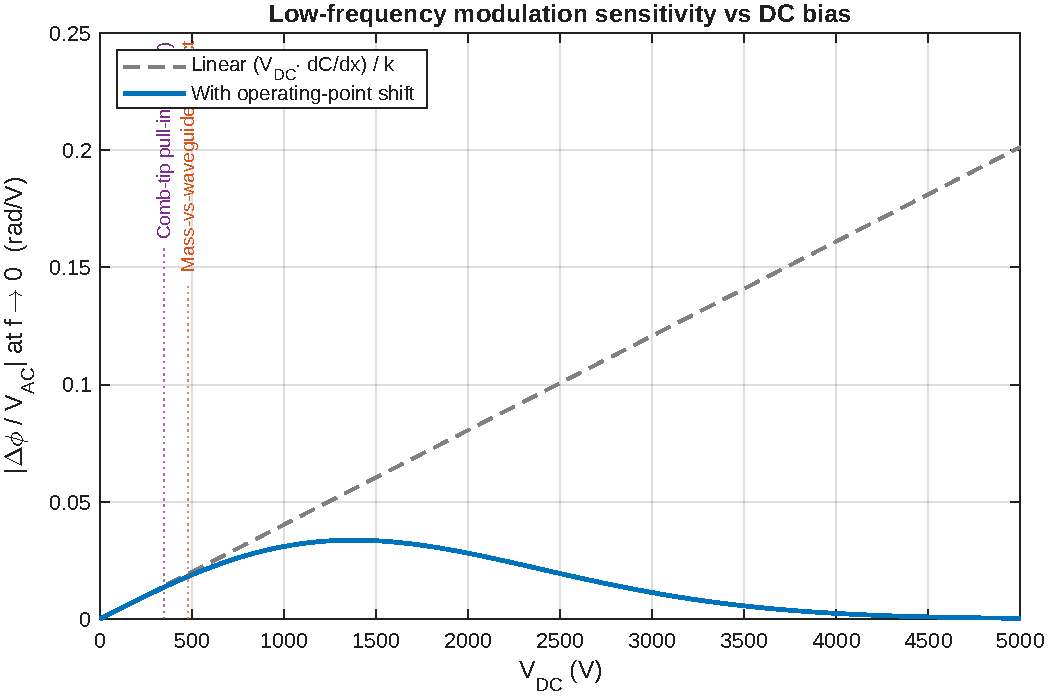
\includegraphics[width=0.78\textwidth]{figures/q8_sens_vs_VDC.pdf}
\caption{Low-frequency modulation sensitivity as a function of $\VDC$.
The dashed grey line is the strict linear $\VDC$ dependence; the solid line
includes the (small) effect of the operating-point shift on $S_{\phi}$.
Practical operation is bounded by comb-tip pull-in at $\sim\!\SI{347}{\volt}$.}
\label{fig:sensVDC}
\end{figure}
